%-----------------------------------------------------------------------------%
\chapter{\topikSatu}
%-----------------------------------------------------------------------------%

%-----------------------------------------------------------------------------%
\section{Pendahuluan}
%-----------------------------------------------------------------------------%

Bahasa pemrograman R adalah salah satu bahasa pemrograman yang digunakan untuk komputasi statistik dan grafis banyak digunakan oleh \f{datascientis} untuk membuat \f{software} untuk mengolah data. R dibuat oleh Ross Ihaka dan Robert Gentleman di University of Auckland. Nama  R kemudian diambil dari huruf pertama dari dua pembuat R.
Pada bahasa R terdapat \f{library} statistik seperti linear dan non-linear model, \f{classification}, \f{time-series­ analysis},dan lain-lain. Selain itu, R didesain agar pengguna mudah dalam memberikan kontribusi bagi pengembangannya, di mana pengguna dapat membuat \f{package} yang dapat digunakan oleh komunitas R lainnya.
R didukung oleh banyak \f{package repository} yang digunakan untuk data manipulasi, perhitungan, dan visualisasi. Dalam suatu \f{package} terdapat fungsi-fungsi untuk memproses data, penyimpanan, operator untuk menghitung \f{array} atau matriks. Bahasa R juga dilengkapi dengan fungsi-fungsi dasar pemrograman lainnya seperti perulangan, rekursif, percabangan dan lain-lain. 

%-----------------------------------------------------------------------------%
\section{Fitur Bahasa R}
%-----------------------------------------------------------------------------%

Bahasa R didukung oleh berbagai fitur diantaranya adalah :
\begin{itemize} 
\item \f{Interpreted language} (dapat dioperasikan menggunakan \f{command line}).
\item Dukungan terhadap beberapa jenis struktur data seperti vektor, matriks, \f{array}, dan \f{data frame} yang merupakan struktur data menyerupai matriks yang mampu menyimpan data dengan tipe yang berbeda.
\item Mendukung fungsi pemrograman prosedural dan berorientasi obyek.
\item Memiliki performa komputasi statistik yang setara dengan Matlab dan Octave.
\item Didukung dengan IDE, beberapa yang populer adalah Rstudio dan Visual Studio.
\end{itemize}

%-----------------------------------------------------------------------------%
\section{Instalasi Bahasa R}
%-----------------------------------------------------------------------------%

%-----------------------------------------------------------------------------%
\subsection{Instalasi Bahasa R pada Linux}
%-----------------------------------------------------------------------------%

Untuk menginstal Bahasa Pemrograman R pada Linux  cukup dengan menuliskan perintah pada terminal seperti berikut
\begin{lstlisting} 
	$ sudo apt-get install r-base
	$ sudo apt-get install r-base-dev #R yang dilengkapi dengan compiler 
\end{lstlisting}
Jika proses instalasi telah selesai, pada terminal Linux, silahkan mengetikan command “R” untuk memulai menulis program R.
\begin{figure}
\centering
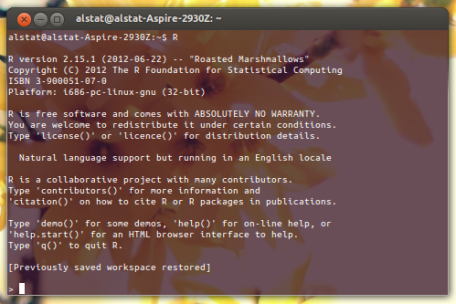
\includegraphics[width=0.7\linewidth]{./pics/instal}
\caption{Tampilan pada \f{command line}}
\label{fig:instal}
\end{figure}


Untuk menggunakan IDE Rstudio pada Ubuntu, RStudio dapat diunduh pada situs \url{https://www.rstudio.com} dan diinstal pada Ubuntu.

%-----------------------------------------------------------------------------%
\subsection{Instalasi Bahasa R pada Windows}
%-----------------------------------------------------------------------------%

Untuk Bahasa R pada Windows, Silahkan unduh berkas instalasi pada situs \url{https://cran.r-project.org/bin/windows/base/} dan instal R-3.x.x-win.exe sebagaimana menginstal \f{software} seperti biasa.

%-----------------------------------------------------------------------------%
\subsection{Instalasi Package Bahasa R}
%-----------------------------------------------------------------------------%
\f{Packages} pada R berisi fungsi-fungsi komputasi statistik tertentu, fungsi grafik, analisa,dan lain-lain yang ditulis menggunakan bahasa R dan dapat juga diintegrasikan dengan bahasa pemrograman lainnya seperti Java, C, C++, FORTRAN. Jumlah \f{package} yang terdapat pada repository CRAN ah 7.801 (Januariy 2016.  Dengan jumlah \f{package} yang sangat besar dan bervariasi, CRAN repositorylam beberapa \f{task} atau idang agar mempermudah pengguna dalam memilih dan menggunakan \f{package} yang sesuai dengan pekerjaannya.

\begin{table}
\caption{Contoh Package}
\label{tab:contoh_package}
\begin{tabular}{|L{4cm}|L{5cm}|L{5cm}|}
\rowcolor[gray]{.9} \hline Task & Keterangan & Contoh nama package \\ 
\hline ChemPhys & Chemometrics and Computational Physic
 & chemCal,simecol, investr,CHNOSZ \\ 
\hline MachineLearning & Machine Learning and Statistical Learning & Caret, rpart, nnet, LogicReg,grpLasso \\ 
\hline MedicalImaging & Medical Image Analysis
 & Dti, tractor.base, DATforDCEMRI, brainwaver,AnalyzeFMRI \\ 
\hline NaturalLanguageProcessing & Natural Language Processing & openNLP,SnowballC,stringi, KoNLP, languageR \\ 
\hline HighPerformanceComputing & High Performance Computing
 & Snow, Rhpc, Rmpi, doRNG,gputools, cudaBayesReg \\ 
\hline 
\end{tabular} 
\end{table}

Cara memasang \f{package} yang ingin diinstal pada bahasa R, yaitu dengan mengetikkan sintaks \textbf{\textquotedblleft install.packages(\textquotedblleft \_nama\_package\_\textquotedblright )\textquotedblright} pada \f{command line} R, atau dapat juga dengan mengunduh \f{file package} terlebih dahulu dan dengan perintah \textbf{install.packages(\textquotedblleft directory\_package\textquotedblright )}, tunggu hingga proses instalasi selesai. Setelah proses instalasi, selesai untuk memanggil \f{package} yang telah terpasang,gunakan perintah \textbf{library(\_nama\_package\_)}, maka fungsi-fungsi yang terdapat pada package tersebut sudah dapat digunakan.

\begin{figure}
\centering
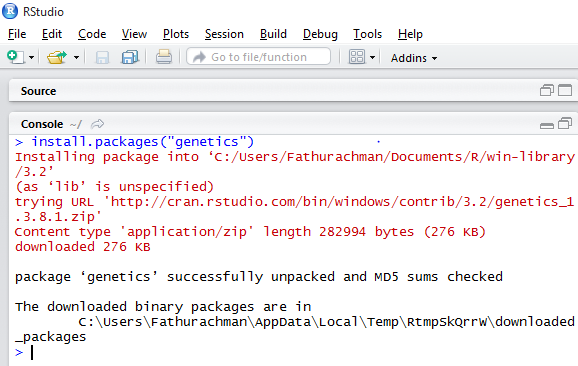
\includegraphics[width=0.7\linewidth]{./pics/instalpackage}
\caption{Cara melakukan instalasi package genetic menggunakan RStudio}
\label{fig:instalpackage}
\end{figure}

\begin{figure}
\centering
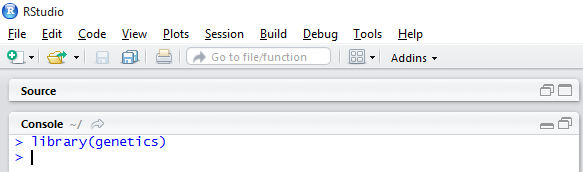
\includegraphics[width=0.7\linewidth]{./pics/importpackage}
\caption{Cara melakukan import package yang telah dipasang}
\label{fig:importpackage}
\end{figure}

\begin{figure}
\centering
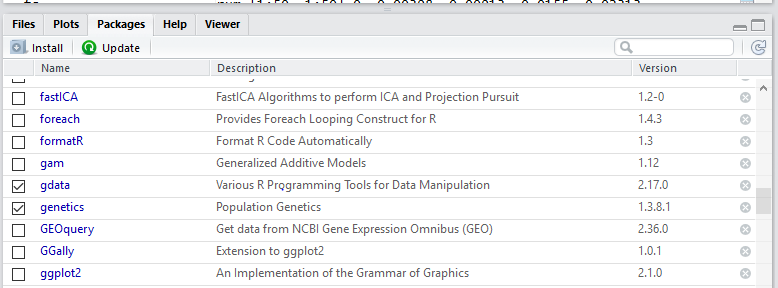
\includegraphics[width=0.7\linewidth]{./pics/daftarpackage}
\caption{Daftar package yang telah terinstal pada lingkungan R}
\label{fig:daftarpackage}
\end{figure}

 
%-----------------------------------------------------------------------------%
\section{Komputasi Paralel pada Bahasa R}
%-----------------------------------------------------------------------------%
Pada dasarnya dalam suatu eksperimen komputasi dibutuhkan suatu proses yang berulang-ulang, hal ini dapat didekati menggunakan fungsi \f{for loop} pada R. Namun jika terdapat komputasi dengan melibatkan data dan proses yang besar, maka komputasi tersebut akan memakan waktu yang sangat lama dan fungsi \f{for loop} akan terlihat sangat lama . Dengan menggunakan fungsi komputasi paralel pada bahasa R yaitu memanfaatkan jumlah \f{core} yang terdapat pada komputer, maka proses komputasi dapat dibagi kepada setiap core processor dan dieksekusi secara paralel untuk menekan waktu komputasi.
Secara Default, R tidak memproses suatu komputasi secara paralel, untuk mengeksekusi suatu proses secara paralel, jumlah core yang tersedia harus didefinisikan dan di daftarkan pada R untuk dibuat suatu kumpulan \f{cluster} agar setiap proses yang dibagi dapat kirim kepada tiap \f{cluster}. Untuk menfasilitasi hal ini, terdapat beberapa \f{package} yang secara efisien mendukung proses paralel.  Namun banyak \f{package} komputasi paralel tidak dapat berjalan di Windows.

\begin{figure}
\centering
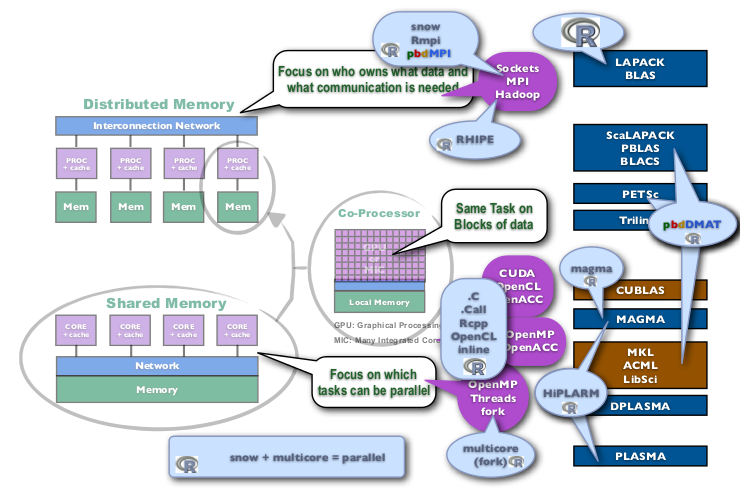
\includegraphics[width=0.7\linewidth]{./pics/parallelpackage}
\caption{Contoh package yang mendukung komputasi paralel \cite{r.schmidt}}
\label{fig:parallelpackage}
\end{figure}

Salah satu \f{package} untuk komputasi paralel adalah \f{package} \textquotedblleft \textbf{parallel}\textquotedblright\space yang disertakan sejak R versi 2.14.  \f{Package} \textquotedblleft \textbf{parallel}\textquotedblright\space merupakan gabungan dari \textquotedblleft \textbf{multicore}\textquotedblright\space yang digunakan pada komputasi paralel dengan \f{shared memory} dan \textquotedblleft \textbf{snow}\textquotedblright\space yang digunakan untuk komputasi paralel dengan \f{distributed memory}.

\begin{table}
\caption{Contoh Fungsi pada Parallel \cite{r.schwendinger}}
\label{tab:contoh_fungsi}
\begin{tabular}{|L{4cm}|L{5cm}|L{5cm}|}
\rowcolor[gray]{.9} \hline Fungsi & Deskripsi & Contoh \\ 
\hline detectCores​ & Mengetahui jumlah inti dari CPU & ncores <- detectCores()​ \\ 
\hline mclapply & Versi paralel lapply (shared memory) & mclapply(1:5, runif, mc.cores = ncores)​ \\ 
\hline makeCluster & Memulai cluster & cl $<$- makeCluster(10, type="MPI")​ \\ 
\hline clusterSetRNGStream & Set seed pada cluster​ & clusterSetRNGStream(cl, 321)​ \\ 
\hline clusterExport & Export variable kepada worker & clusterExport(cl, list(a=1:10, x=runif(10)))​ \\ 
\hline clusterEvalQ & Evaluasi ekspresi pada worker & clusterEvalQ(cl, {x $<$- 1:3​
myFun $<$- function(x) runif(x)}) \\ 
\hline clusterCall & Memanggil fungsi pada semua worker & clusterCall(cl, function(y) 3 + y, 2)​ \\ 
\hline parLapply & Versi paralel dari lapply (distributed memory) & parLapply(cl, 1:100, Sys.sleep)​ \\ 
\hline parLapplyLB & parLapply dengan load balancing & parLapplyLB(cl, 1:100, Sys.sleep)​ \\ 
\hline stopCluster & Menghentikan cluster & stopCluster(cl) \\ 
\hline 
\end{tabular} 
\end{table}

\f{Package} \textquotedblleft \textbf{forEach}\textquotedblright\space merupakan \f{package} yang digunakan untuk komputasi paralel dengan menyediakan \f{single interface} untuk beberapa jenis \f{backend}, salah satunya adalah \textquotedblleft \textbf{doParallel}\textquotedblright.

Contoh \textquotedblleft \textbf{forEach}\textquotedblright\space menggunakan \textquotedblleft \textbf{multicore}\textquotedblright\space \f{shared memory}

\begin{lstlisting}
	library(doParallel)​
	registerDoParallel(cores=ncores)​
	foreach(i=1:2) %dopar% Sys.getpid()​
\end{lstlisting}

Contoh \textquotedblleft \textbf{forEach}\textquotedblright\space menggunakan \textquotedblleft \textbf{snow}\textquotedblright\space \f{distributed memory}

\begin{lstlisting}
	library(doParallel)​
	cl <- makeCluster(ncores)​
	registerDoParallel(cl=cl)​
	foreach(I=1:2) %dopar% Sys.getpid()​
	stopCluster(cl)​
\end{lstlisting}

Untuk membuat proses paralel pada suatu komputasi dapat mengikuti petunjuk dari code dibawah ini

\begin{lstlisting}
	library(doParallel)
	# Menampilkan Jumlah Core yang terdapat pada Komputer
	detectCores()
	## [1] 4
	# Membuat Cluster cl dengan jumlah cluster sebanyak 3
	cl <- makeCluster(3)
	# Melakukan Registrasi Cluster sebagai Backend
	registerDoParallel(cl)
	# Menampilkan Jumlah Prosessor yang digunakan untuk komputasi paralel
	getDoParWorkers()
	## [1] 3
\end{lstlisting}

Prinsip kerja komputasi paralel, membagi masalah menjadi sub-masalah, lakukan eksekusi terhadap setiap sub-masalah secara paralel, kemudian menggambungkan setiap hasil eksekusi. Berikut adalah contoh potongan program secara sekuensial.

\begin{lstlisting}
	#Number of iteration
	iters <- 100000
	#vector for appending output
	ls <-vector('list', length = iters)
	start <- Sys.time()
	#loop
	for (i in 1:iters) {
	  #Counter
	  #cat(i,'\n')
	  to.ls<-rnorm(1e6)
	  to.ls<-summary(to.ls)
	  ls[[i]]<-to.ls
	}
	#End time
	print(Sys.time()-start)
\end{lstlisting}

Dan perbandingannya dengan program secara paralel.

\begin{lstlisting}
  iters<-10000
  #setup parallel backend to use 3 processors
  cl<-makeCluster(3)
  registerDoParallel(cl)
  #start time
  strt<-Sys.time()
  #loop
  ls<-foreach(icount(iters)) %dopar% {
    to.ls<-rnorm(1e6)
    to.ls<-summary(to.ls)
    to.ls
  }
  print(Sys.time()-strt)
  stopCluster(cl)
\end{lstlisting}

Pada potongan secara sequential dan paralel, proses yang dilakukan adalah membagi sampel data dengan jumlah 1.000.000 data, seacara distribusi normal. Yang diulang sebanyak 100000 iterasi.  Terlihat bahwa pada proses sequential, hanya menggunakan fungsi for loop, sedangkan pada proses paralel terlebih dahulu dibuat cluster sebanyak 3, kemudian pada proses melakukan sampel data, proses tersebut dilakukan secara paralel. Syntax \textbf{\%dopar\%} mengindikasikan bahwa code selanjutnya akan dikerjakan secara parallel yang dikirimkan kepada tiap cluster.  Perbandingan yang dilakukan yaitu melihat hubungan antara proses yang dilakukan dan waktu yang dibutuhkan. Hasil dari eksekusi program diatas dapat dilihat pada gambar dibawah ini.

\begin{figure}
\centering
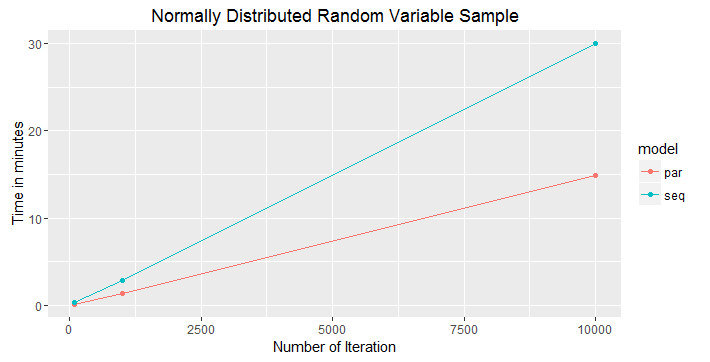
\includegraphics[width=0.7\linewidth]{./pics/perbandingan}
\caption{Perbandingan program sekuensial dengan paralel}
\label{fig:perbandingan}
\end{figure}

Dari hasil Eksekusi diatas terlihat bahwa terjadi speed up 2 kali lipat terhadap proses paralel. Khusus pada komputasi paralel pada R, terdapat dua jenis package yang mendukung proses paralel, tipe pertama adalah package dengan paralel implisit yang setiap fungsinya telah mendukung proses paralalel, artinya ketika menggunakan fungsi pada package tersebut, maka proses paralalel akan dilakukan tanpa pengguna terlebih dahulu membuat cluster dari jumlah core yang tersedia. Tipe yang kedua adalah package paralel secara eksplisit, dimana proses paralel harus didefinisikan terlebih dahulu, dengan menentukan jumlah cluster, serta problem dan proses yang akan dieksekusi secara paralel.

%-----------------------------------------------------------------------------%
\subsection{Komputasi Paralel dengan GPU pada Bahasa R}
%-----------------------------------------------------------------------------%

GPU atau Graphical Processing Unit, adalah merupakan single-chip processor yang melakukan komputasi khusus untuk aplikasi 3D.  Berbeda dengan CPU yang hanya memiliki beberapa core pada satu chip, GPU memiliki ratusan-bahkan ribuan core dalam satu chip. Karena sebagian besar proses komputasi pada GPU mencakup operasi vektor dan matriks, maka GPU dapat digunakan untuk mengeksekusi proses lain yang berbeda dengan pemrosesan pada graphics. Dalam hal ini GPU digunakan untuk melakukan komputasi non-graphical process, seperti menjalankan algoritma, komputasi FFT, persamaan linear.

Untuk mengakses GPU menggunakan R, terdapat dua cara yaitu :

\begin{itemize}
\item Menggunakan package yang tersedia oleh CRAN.
\item Mengakses GPU melalui CUDA Library / CUDA Accelerated Programming Language C, C++, FORTRAN.
\end{itemize}

\begin{figure}
\centering
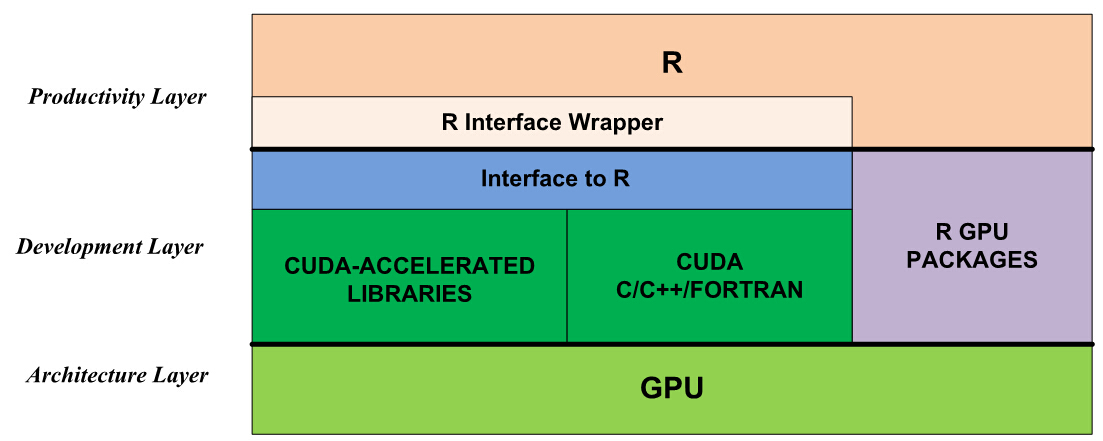
\includegraphics[width=0.7\linewidth]{./pics/skemaaksesgpu}
\caption{Skema akses bahasa R terhadap GPU}
\label{fig:skemaaksesgpu}
\end{figure}

Untuk menggunakan package yang mendukung komputasi GPU dapat menggunakan package pada tabel berikut.

\begin{table}
\caption{Daftar Package yang mendukung fungsi GPU}
\label{tab:contoh_gpu}
\begin{tabular}{|L{5cm}|L{9cm}|}
\rowcolor[gray]{.9} \hline Nama Package
 & Keterangan \\ 
\hline gputools & Package yang menyediakan fungsi-fungsi algoritma data mining yang diintegrasikan dengan library CUDA dan CUBLAS, dengan didukung oleh Nvidia GPU, akan menghasilkan komputasi yang efisien.
 \\ 
\hline cudabayesReg & Package yang menyediakan fungsi rhierLinearModel dari package bayesm menggunakan library CUDA untuk mendukung High Performance Statistical Analysis dari FMRI Voxels \\ 
\hline gcbd & Package menggunakan standar library  BLAS dan GPU
 \\ 
\hline OpenCL
 & Package yang menyediakan Interface dari R – OPEN CL \\ 
\hline HiPLARM & Package yang menyediakan fungsi Linear Algebra yang mendukung multicore / GPU menggunakan library PLASMA/MAGMA  \\ 
\hline gmatrix & Package yang menyediakan fungsi operasi matriks dan vektor menggunakan GPU \\ 
\hline gpuR & Menyediakan fungsi untuk mengakses GPU dan VCL untuk memproses objek pada R seperti matrik dan vektor tanpa menggunakan bahasa Open CL  \\ 
\hline rgpu & Package yang menyediakan fungsi untuk mempercepat proses analisis pada Bioinformatics menggunakan GPU \\ 
\hline 
\end{tabular} 
\end{table}

Contoh program R menggunakan GPU :

\begin{lstlisting}
	library(gputools)
	gpu.matmult <- function(n) {
    A <- matrix(runif(n * n), n ,n)
    B <- matrix(runif(n * n), n ,n)
    tic <- Sys.time()
    C <- A %*% B
    toc <- Sys.time()
    comp.time <- toc - tic
    cat("CPU: ", comp.time, "\n")
    tic <- Sys.time()
    C <- gpuMatMult(A, B)
    toc <- Sys.time()
    comp.time <- toc - tic
    cat("GPU: ", comp.time, "\n")
}
\end{lstlisting}

Simulasi program diatas menggunakan \f{package} gputools, dengan melakukan deklarasi fungsi untuk melakukan perkalian matriks. Fungsi tersebut memberikan keluaran berupa hasil waktu CPU dan GPU yang dibutuhkan untuk melakukan perkalian matriks. Dengan menggunakan fungsi gpuMatMul(A,B) pada \f{package} gputools, proses perkalian matriks A dan B dilakukan dengan menggunakan GPU.

Hasil eksekusi program terlihat bahwa, untuk ukuran matriks yang kecil, CPU melakukan komputasi  lebih baik dari GPU, namun untuk ukuran matriks yang lebih besar dari 2000, maka terlihat GPU jauh lebih cepat dibandingkan CPU.

%-----------------------------------------------------------------------------%
\subsection{CUDA pada Bahasa R}
%-----------------------------------------------------------------------------%

Mengakses GPU dengan menggunakan \f{library} CUDA dengan mengintegrasikan menggukan bahasa C, pastikan bahwa pada komputer anda dilengkapi dengan hardware GPU Nvidia, dan telah terinstal CUDA. Langkah-Langkah untuk menggunakan library CUDA adalah sebagai berikut :

\begin{itemize}
\item Membuat \f{interface} sebagai penghubung antara R dan library CUDA.
\item \f{Compile} dan membuat \f{link shared object}. \f{Shared object} berisi fungsi-fungsi pada bahasa C yang akan diakses oleh R.
\item \f{Load shared object}.
\item Eksekusi dan tes.
\end{itemize}

%-----------------------------------------------------------------------------%
\subsubsection{Membuat Interface}
%-----------------------------------------------------------------------------%

\begin{lstlisting}
#include 
#include <cufft.h>
/* This function is written for R to compute 1D FFT.
   n - [IN] the number of complex we want to compute
   inverse - [IN] set to 1 if use inverse mode
   h_idata_re - [IN] input data from host (R, real part)
   h_idata_im - [IN] input data from host (R, imaginary part)
   h_odata_re - [OUT] results (real) allocated by caller
   h_odata_im - [OUT] results (imaginary) allocated by caller
*/
extern "C"
void cufft(int *n, int *inverse, double *h_idata_re,
           double *h_idata_im, double *h_odata_re, double *h_odata_im)
{
  cufftHandle plan;
  cufftDoubleComplex *d_data, *h_data;
  cudaMalloc((void**)&d_data, sizeof(cufftDoubleComplex)*(*n));
  h_data = (cufftDoubleComplex *) malloc(sizeof(cufftDoubleComplex) * (*n));

  // Convert data to cufftDoubleComplex type
  for(int i=0; i< *n; i++) {
    h_data[i].x = h_idata_re[i];
    h_data[i].y = h_idata_im[i];
  }
 
  cudaMemcpy(d_data, h_data, sizeof(cufftDoubleComplex) * (*n), 
             cudaMemcpyHostToDevice);
  // Use the CUFFT plan to transform the signal in place.
  cufftPlan1d(&plan, *n, CUFFT_Z2Z, 1);
  if (!*inverse ) {
    cufftExecZ2Z(plan, d_data, d_data, CUFFT_FORWARD);
  } else {
    cufftExecZ2Z(plan, d_data, d_data, CUFFT_INVERSE);
  }

  cudaMemcpy(h_data, d_data, sizeof(cufftDoubleComplex) * (*n), 
  cudaMemcpyDeviceToHost);
  // split cufftDoubleComplex to double array
  for(int i=0; i<*n; i++) {
    h_odata_re[i] = h_data[i].x;
    h_odata_im[i] = h_data[i].y;
  }
 
  // Destroy the CUFFT plan and free memory.
  cufftDestroy(plan);
cudaFree(d_data);
 free(h_data);
}
\end{lstlisting}

\f{Interface} diatas  memasukan  \f{header file} “R.h” dan cufft.h. ditambahkan dengan fungsi cufft untuk melakukan proses Fast Fourier Transform dengan menggunakan CUDA. Sintaks “extern C” membuat fungsi pada \f{interface} ini dapat diakses melalui R. Fungsi tersebut menerima 4 argumen masukan dan 2 keluaran yang hasil komputasinya akan dikembalikan pada R.

%-----------------------------------------------------------------------------%
\subsubsection{Compile dan Hubungkan Shared Object}
%-----------------------------------------------------------------------------%

Setelah menulis sebuah \f{interface}, langkah selanjutnya adalah mengcompile \f{interface} tersebut agar dapat digunakan oleh R, sesuai dengan contoh dibawah ini.

\begin{lstlisting}
nvcc -O3 -arch=sm_35 -G -I/usr/local/cuda/r65/include 
         -I/home/patricz/tools/R-3.0.2/include/ 
         -L/home/patricz/tools/R/lib64/R/lib -lR 
         -L/usr/local/cuda/r65/lib64 -lcufft 
         --shared -Xcompiler -fPIC -o cufft.so cufft-R.cu
\end{lstlisting}
%-----------------------------------------------------------------------------%
\subsubsection{Menggunakan Shared Object}
%-----------------------------------------------------------------------------%

Untuk menggunakan \f{shared object} yang telah dibuat melalui \f{interface}, maka dapat dibuat sebuah fungsi pada R untuk mengakses \f{shared object} tersebut, seperti dibawah ini.

\begin{lstlisting}
cufft1D <- function(x, inverse=FALSE)
{
  if(!is.loaded("cufft")) {
    dyn.load("cufft.so")
  }
  n <- length(x)
  rst <- .C("cufft",
  as.integer(n),
  as.integer(inverse),
  as.double(Re(z)),
  as.double(Im(z)),
  re=double(length=n),
  im=double(length=n))
  rst <- complex(real = rst[["re"]], imaginary = rst[["im"]])
  return(rst)
}
\end{lstlisting}

Fungsi R diatas memanggil file \f{shared object}  “cufft.so” yang akan digunakan pada R. Sintaks “.C(“cufft”,...)” yaitu memanggil fungsi cufft pada \f{shared object} untuk digunakan operasi Fast Fourier Transform.

%-----------------------------------------------------------------------------%
\subsubsection{Eksekusi dan Tes}
%-----------------------------------------------------------------------------%

\begin{lstlisting}
source("wrap.R")
> num <- 4
> z <- complex(real = stats::rnorm(num), imaginary = stats::rnorm(num))
> cpu <- fft(z)
[1] 1.140821-1.352756i -3.782445-5.243686i 1.315927+1.712350i -0.249490+1.470354i
> gpu <- cufft1D(z)
[1] 1.140821-1.352756i -3.782445-5.243686i 1.315927+1.712350i -0.249490+1.470354i
> cpu <- fft(z, inverse=T)
[1] 1.140821-1.352756i -0.249490+1.470354i 1.315927+1.712350i -3.782445-5.243686i
> gpu <- cufft1D(z, inverse=T)
[1] 1.140821-1.352756i -0.249490+1.470354i 1.315927+1.712350i -3.782445-5.
\end{lstlisting}

Hasil yang terlihat diatas, bahwa perhitungan CPU dan GPU menghasilkan waktu yang sama. Namun jika menggunakan hardware yang berbeda, maka akan terlihat perbedaan yang signifikan.

\begin{figure}
\centering
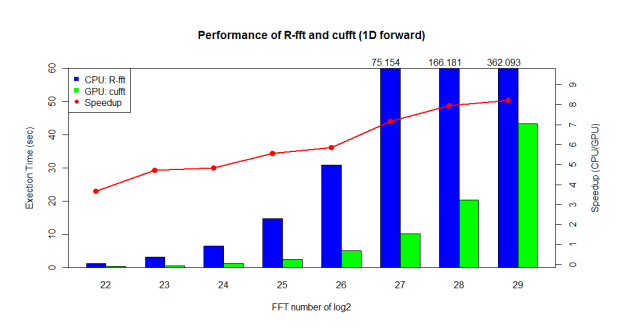
\includegraphics[width=0.7\linewidth]{./pics/hasileksperimen}
\caption{Hasil eksperimen}
\label{fig:hasileksperimen}
\end{figure}

Fungsi R dijalankan pada 8-core Intel® Xeon® CPU (E5-2609 @ 2.40GHz / 64GB RAM) dan NVIDIA GPU (Tesla K20Xm with 6GB device memory ) terlihat bahwa cufft memberikan 3x-8x speedup dibandingkan fungsi FFT pada R.